\begin{frame}{Resultados}
  \begin{itemize}
    \item Primeiramente como resultado da parte de \textit{hardware} podemos apresentar a formulação dos circuitos dos módulos \textbf{CCM} e \textbf{TCM};
  \end{itemize}

\end{frame}
\begin{frame}{Resultados}

  \begin{figure}[H]
    \centering
    \caption{Protótipo montado.}
    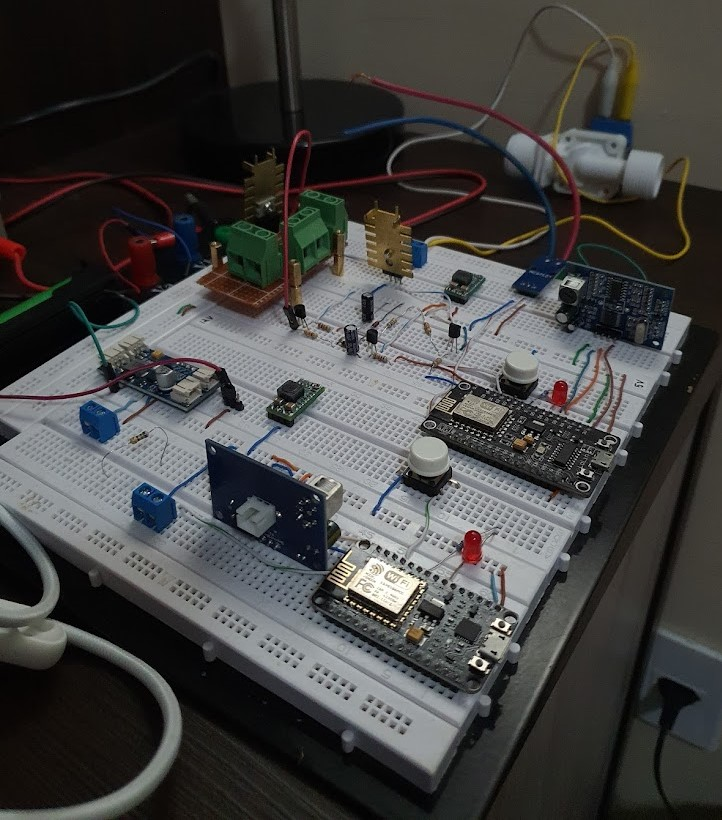
\includegraphics[width=0.4\textwidth]{figuras/esquema_protoboard.jpg}
    \caption*{\tiny{Fonte: Própria.}}
    \label{fig:figma_plan_desktop}
  \end{figure}

\end{frame}

\begin{frame}{Resultados}

  \begin{itemize}
    \item Também foram desenvolvidos os esquemáticos dos dois módulos, levando em consideração todas as ligações: circuitos de alimentação, sensoriamento e comunicação. Esse resultado garante futuras implementações de \textit{layout's 3D} e confecção das placas de circuito impresso.
  \end{itemize}

\end{frame}

\begin{frame}{Resultados}

  \begin{figure}[H]
    \centering
    \caption{Esquemático do módulo CCM implementado no Kicad.}
    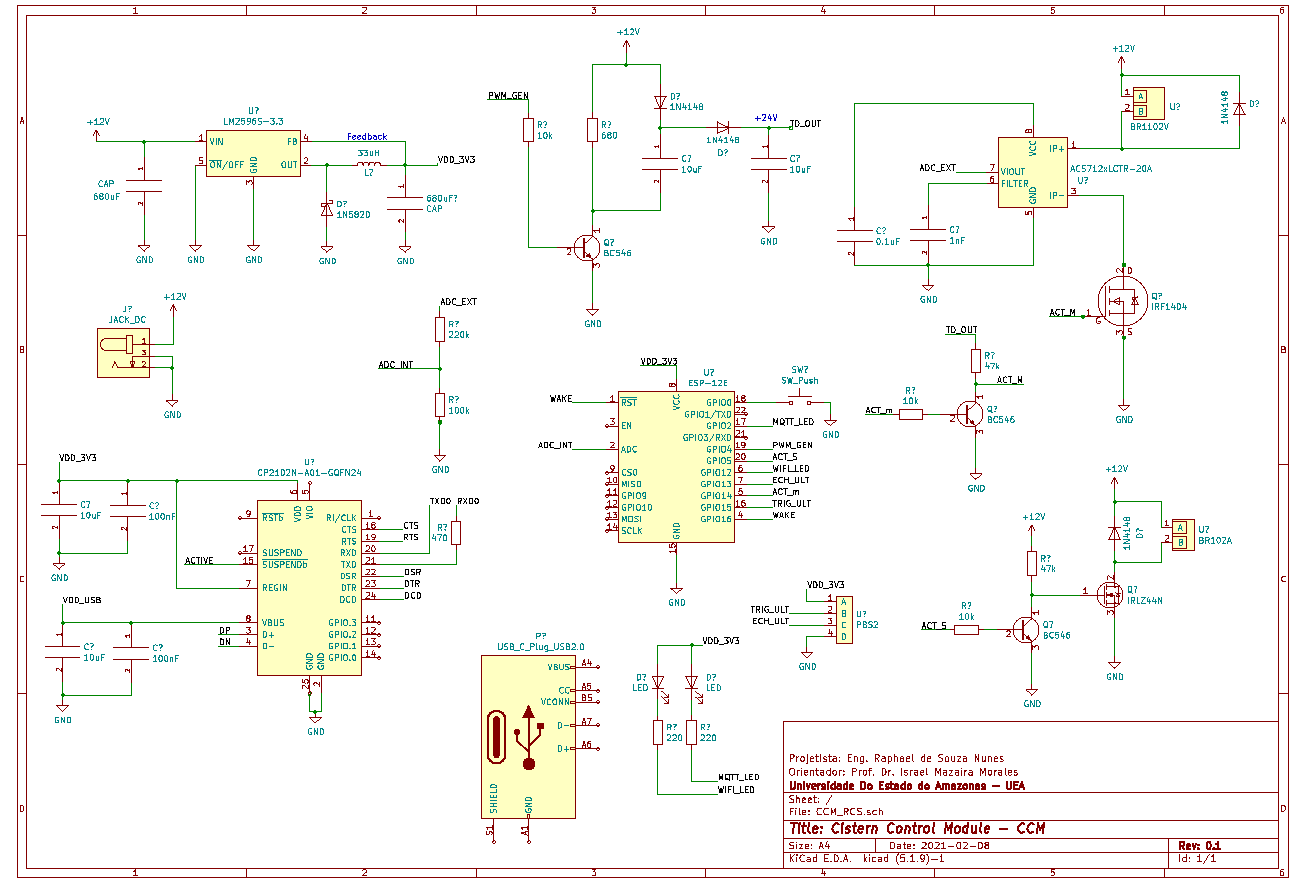
\includegraphics[width=0.7\textwidth]{figuras/kicad_ccm.png}
    \caption*{\tiny{Fonte: Própria.}}
    \label{fig:kicad_ccm}
  \end{figure}

\end{frame}

\begin{frame}{Resultados}

  \begin{itemize}
    \item No quesito de \textit{firmware}, alcançou-se todas as funcionalidades propostas, gerando um código estável e escalável para projetos reais.
  \end{itemize}

\end{frame}

\begin{frame}{Resultados}
  \begin{figure}[H]
    \centering
    \caption{Versão final do código do \textit{firmware}}
    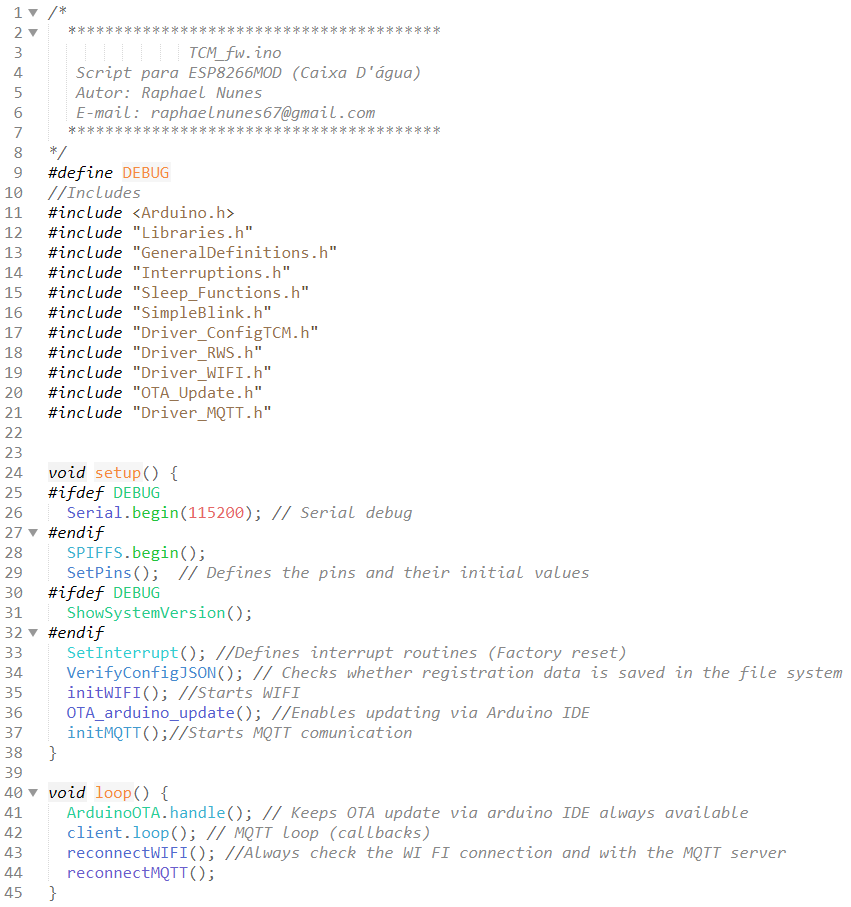
\includegraphics[width=0.5\textwidth]{figuras/tcm_main.png}
    \caption*{\tiny{Fonte: Própria.}}
    \label{fig:tcm_main}
  \end{figure}
\end{frame}

\begin{frame}{Resultados}

  \begin{itemize}
    \item Por fim, também obtivemos como resultado a elaboração de telas utilizando as tecnologias propostas, atingindo o objetivo de relacionar o \textit{software} com as camadas de \textit{firmware} e \textit{hardware}.
  \end{itemize}
\end{frame}

\begin{frame}{Resultados}
  \begin{figure}[H]
    \centering
    \caption{Implementação da aplicação \textit{desktop}.}
    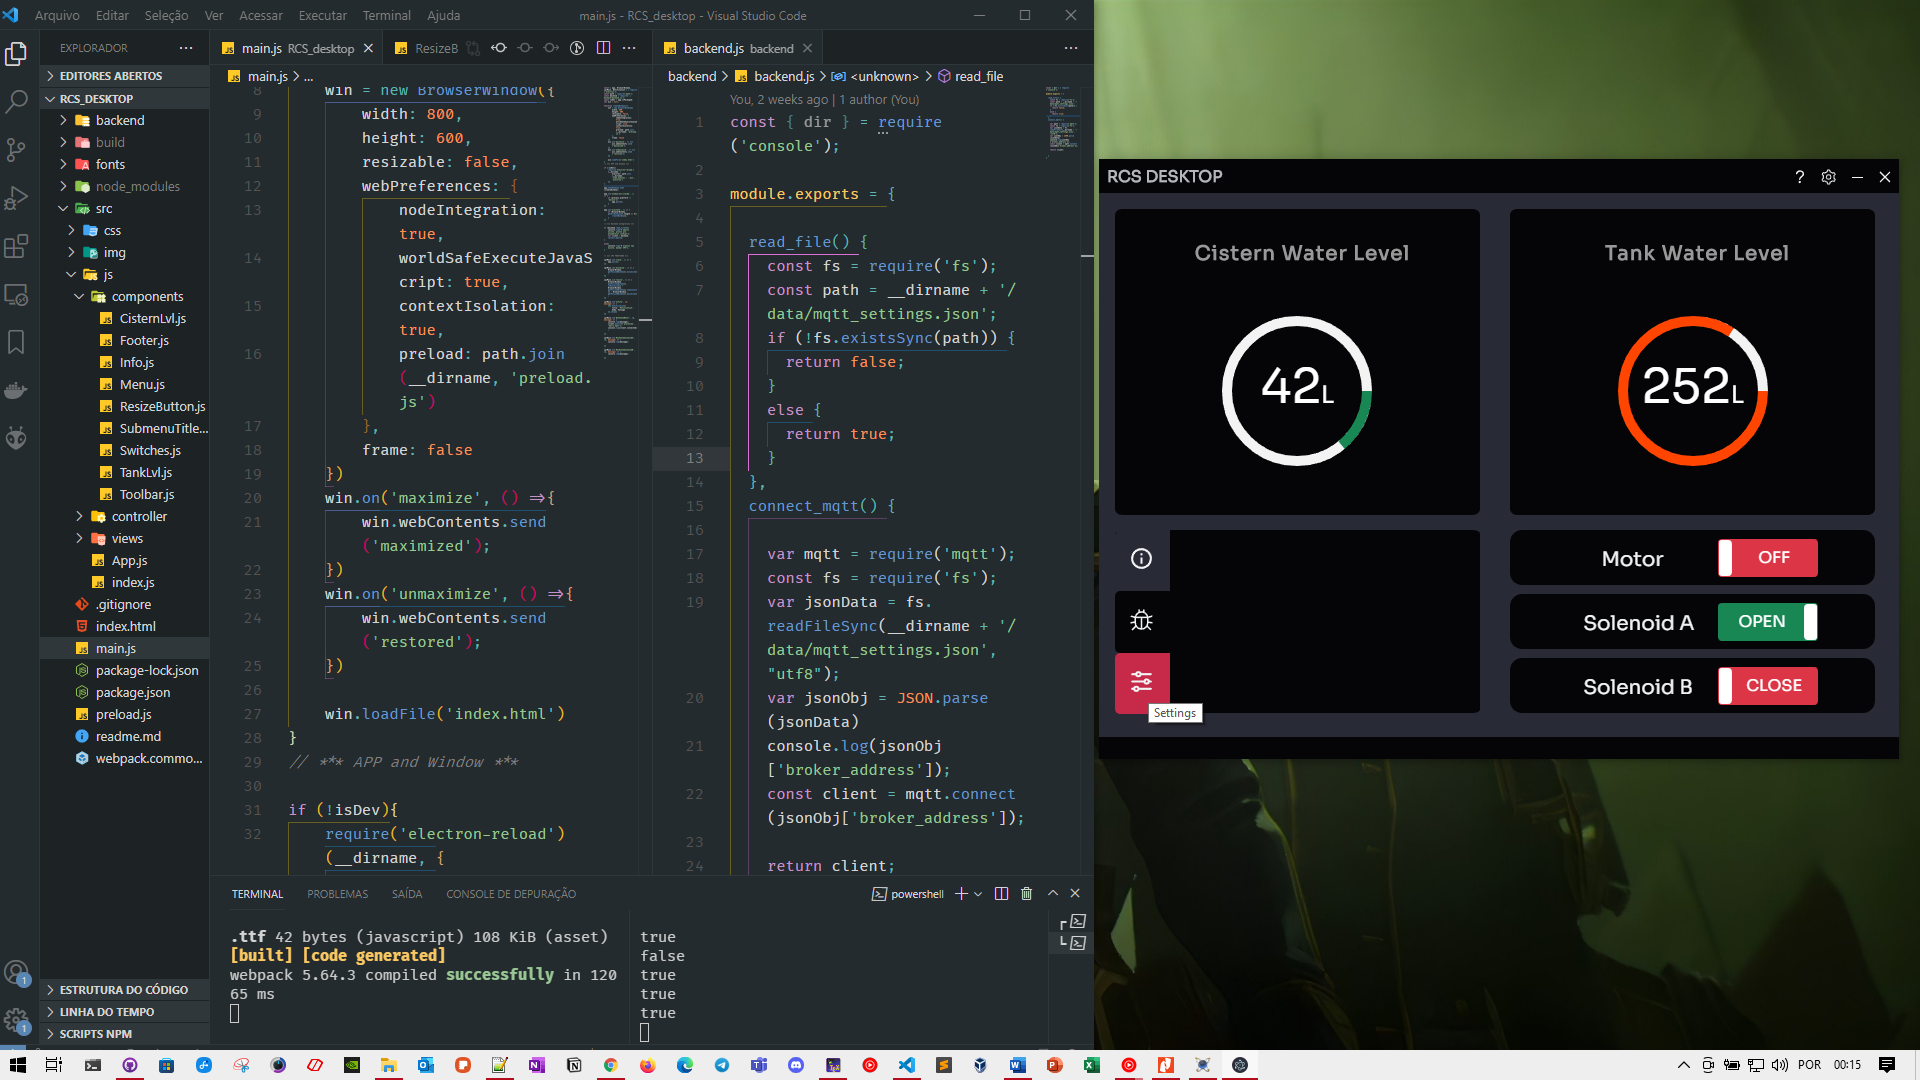
\includegraphics[width=0.6\textwidth]{figuras/rcs_desktop.png}
    \caption*{\tiny{Fonte: Própria.}}
    \label{fig:tela_desktop}
  \end{figure}
\end{frame}

\begin{frame}{Resultados}
  \begin{figure}[H]
    \centering
    \caption{Implementação da aplicação \textit{mobile}.}
    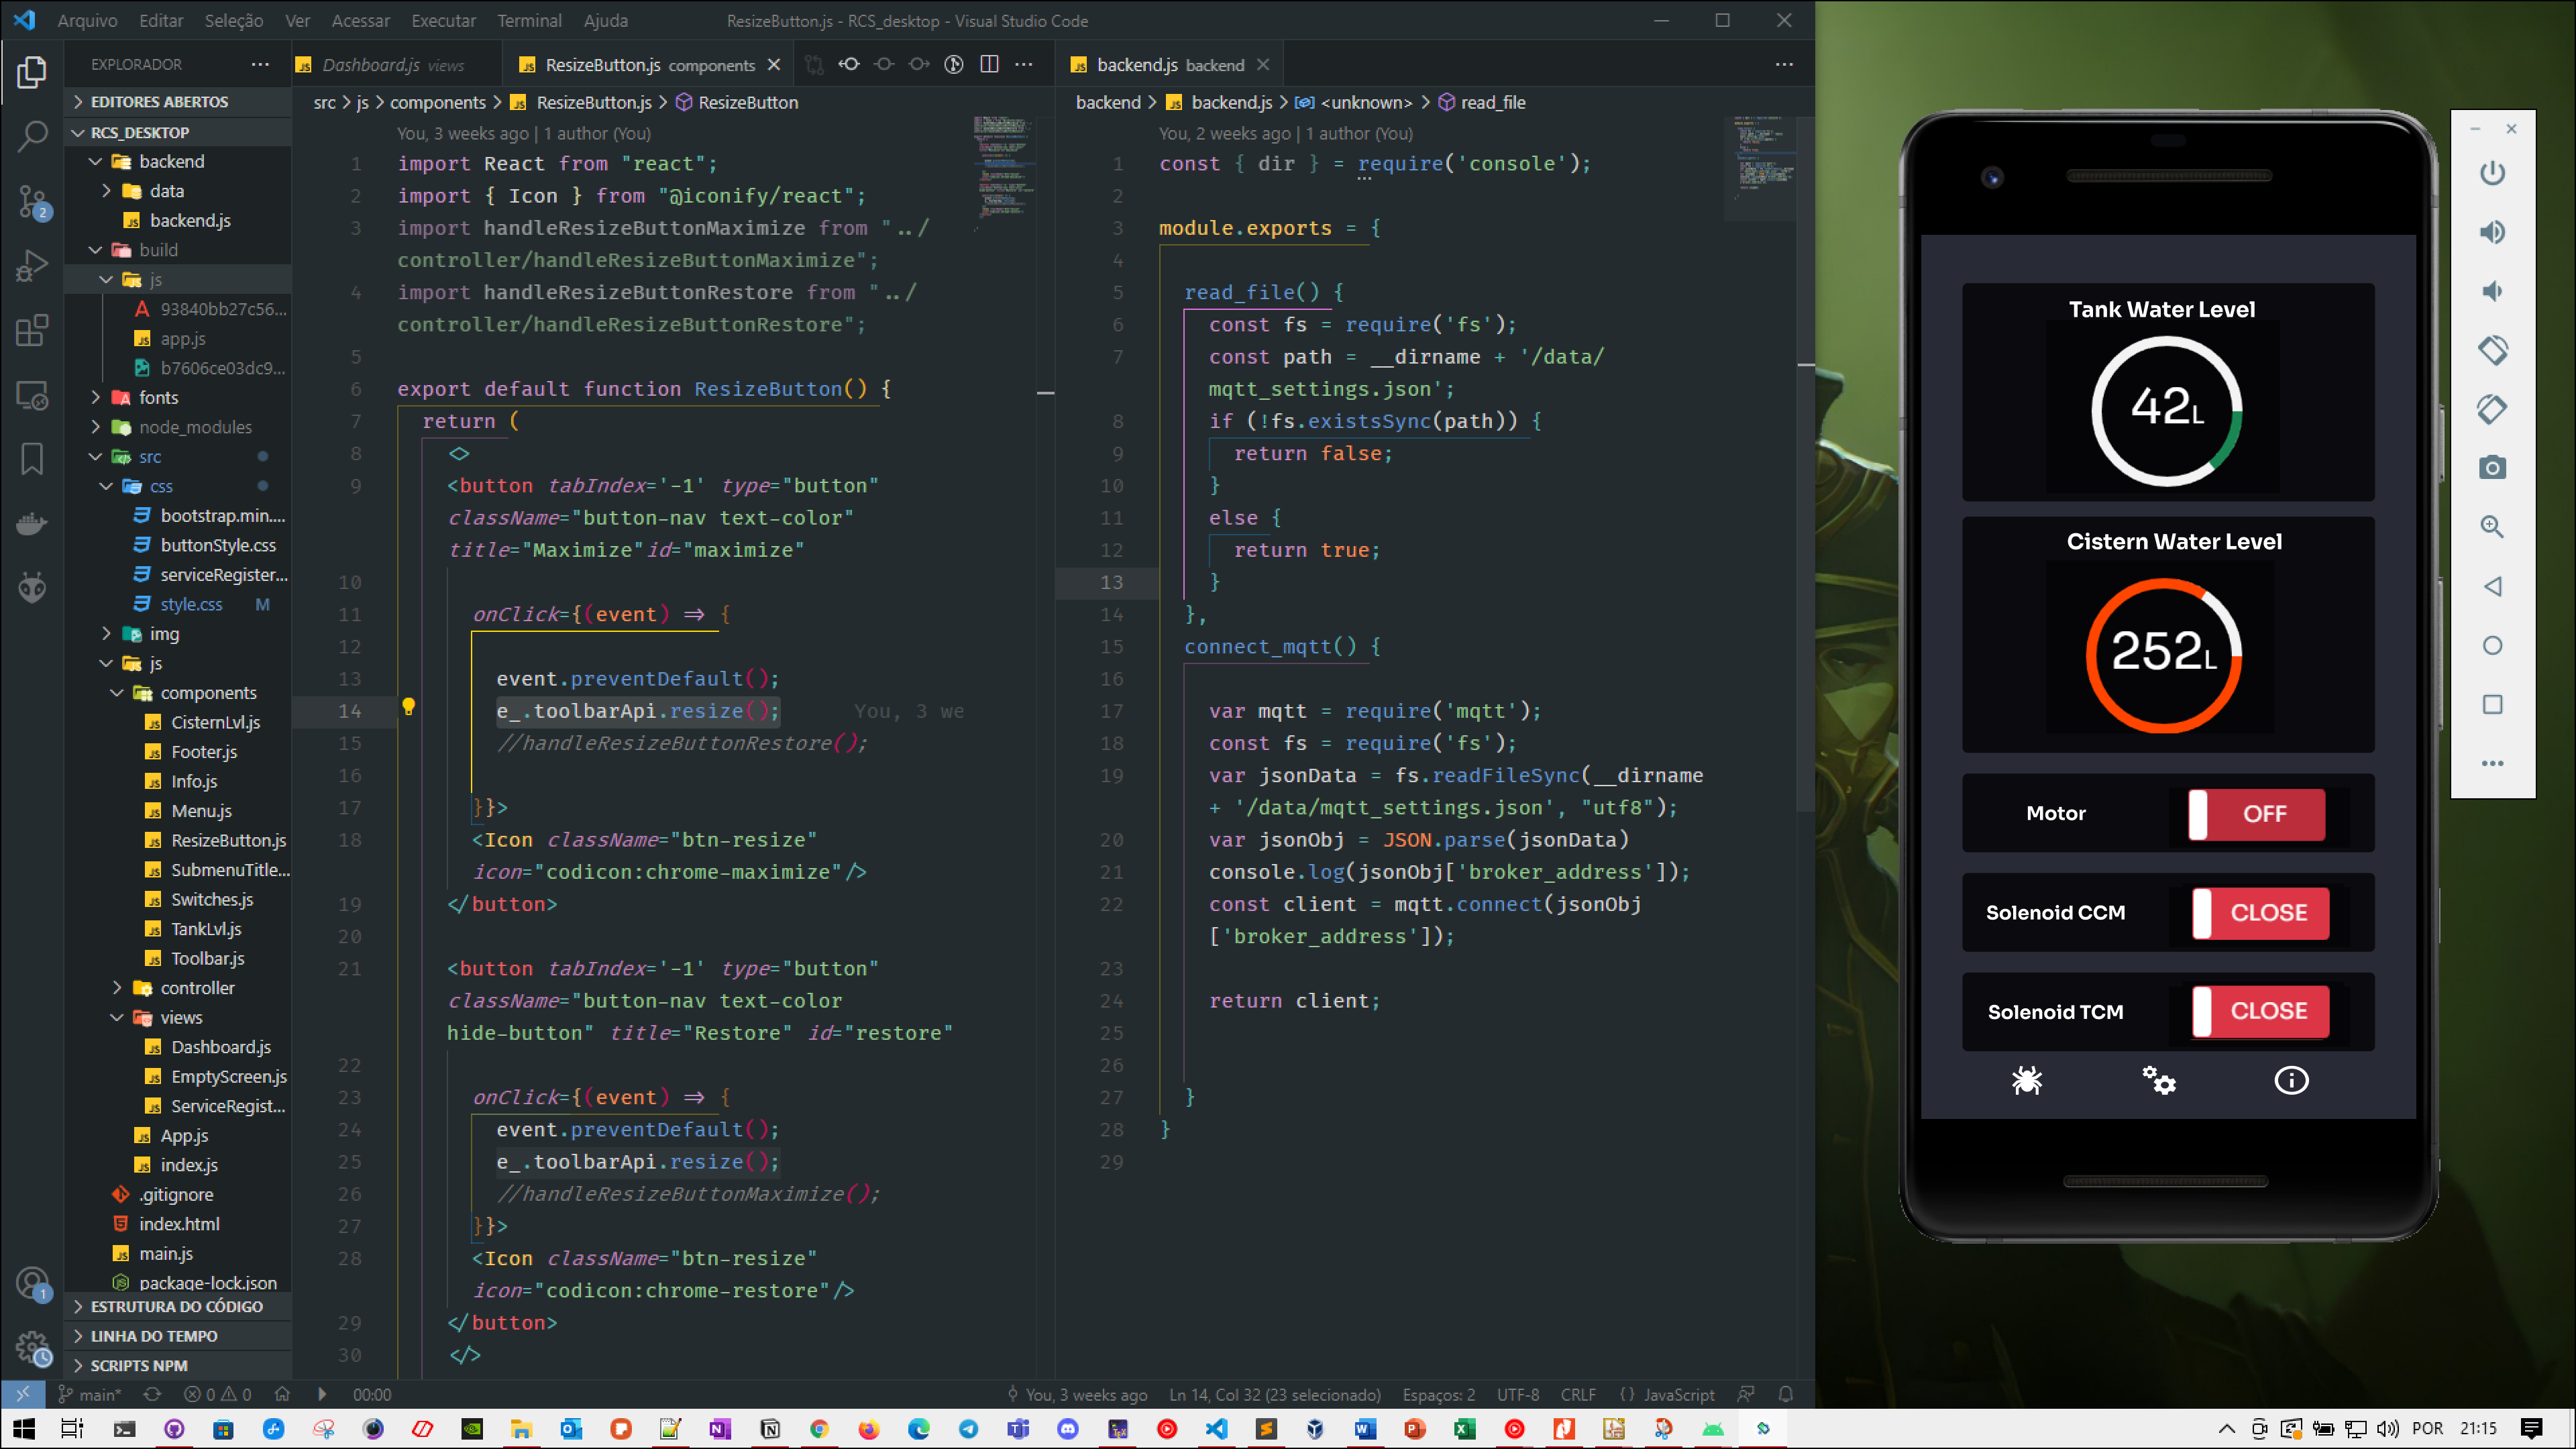
\includegraphics[width=0.6\textwidth]{figuras/rcs_mobile.png}
    \caption*{\tiny{Fonte: Própria.}}
    \label{fig:tela_mobile}
  \end{figure}
  
\end{frame}